\section{Detector Calibrations}
% TODO: make sure I have links to calibration guides for each system
\subsection{Hodoscopes}
The calibration procedure for the hodoscopes consists of determining a set of
timing corrections applied to the raw times $t_{raw}$ generated by
discriminators fed into TDCs.
The general form of a corrected TDC time for one end of a scintillator paddle
is
\begin{equation}
    t_{corr} = t_{raw} - t_{TW} - t_{cable} - t_{prop} - t_{\lambda}
\end{equation}

\begin{itemize}
    \item \textbf{Timewalk corrections} $t_{TW}$

Timewalk refers to the correlation between
the amplitude of an analog signal fed into a leading-edge, fixed-threshold discriminator
and the time the signal rises rises above the discriminator's threshold.
As seen in Fig~\ref{fig:pooser_timewalk}, pulses with a smaller amplitude cross
a fixed threshold at later times despite starting at the same time.

\begin{figure}[!h]
    \centering
    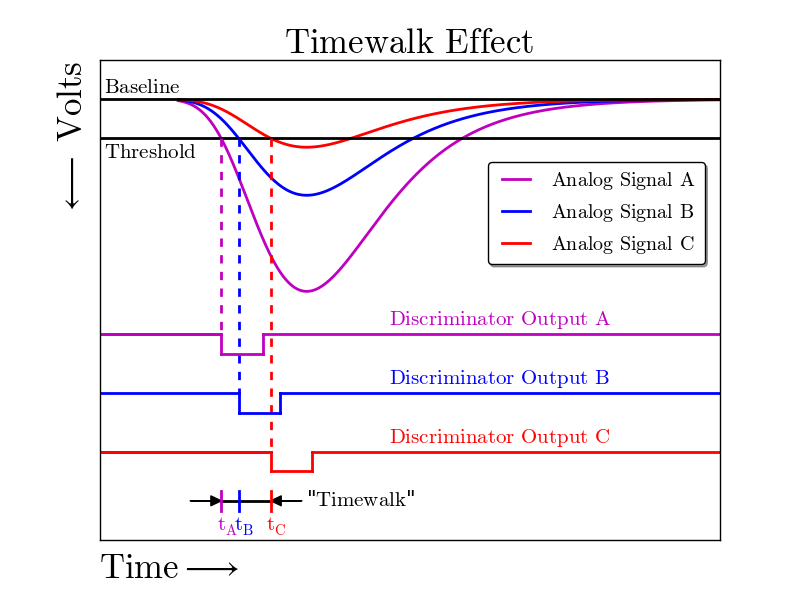
\includegraphics[width=0.6\textwidth]{chap4/pooser_timewalk.png}
    \caption{
            An illustration of the timewalk effect.
            Pulses with a smaller amplitude cross the fixed threshold at a
            later time.
            The TDCs in the Hall C DAQ are prone to this effect.
            }
    \label{fig:pooser_timewalk}
\end{figure}

Fortunately, the fADCs are not prone to this effect so the pulse time recorded
by an fADC can be used to correct the corresponding TDC time.
The fADC pulse time is determiend by a constant fraction discriminator (CFD)
algorithm that finds the time,
to a precision of \SI{62.5}{\pico\second},
at which the pulse reaches 50\% of its maximum amplitude.
This algorithm is illustrated in Fig~\ref{fig:pooser_cfd}, and a comparison of
pulse times of varying amplitudes is shown in Fig~\ref{fig:pooser_notimewalk}.

\begin{figure}[!h]
    \centering
    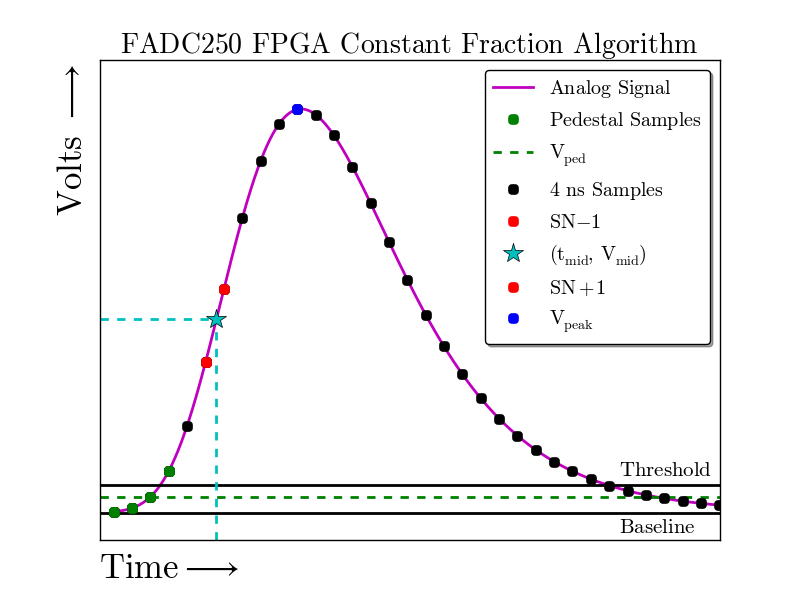
\includegraphics[width=0.6\textwidth]{chap4/pooser_cfd.png}
    \caption{
            An illustration of the fADCs' CFD algorithm.
            The algorithm calculates the pedestal amplitude $V_{ped}$ with a
            fixed-threshold discriminator.
            It then calculates the half-amplitude $V_{mid}=(V{peak}-V_{ped})/2$
            and determines which two samples $SN-1$ and $SN+1$ lie on either
            side of $V_{mid}$.
            The fADCs' coarse sampling rate is \SI{250}{\mega\hertz}, yielding
            \SI{4}{\nano\second} between the two samples.
            This time is divided into 64 subsamples of \SI{62.5}{\pico\second}
            each, and the time $t_{mid}$ corresponding to $V_{mid}$ is found by
            linear interpolation..
            }
    \label{fig:pooser_cfd}
\end{figure}

\begin{figure}[!h]
    \centering
    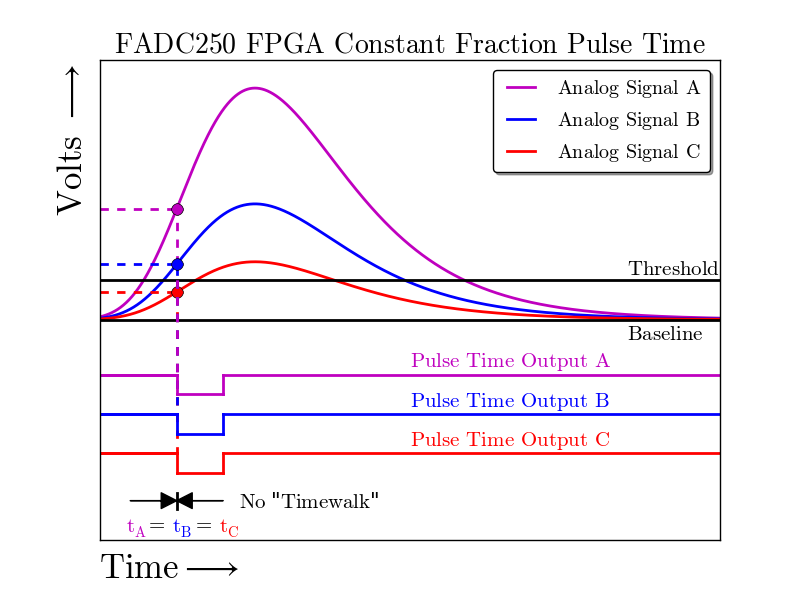
\includegraphics[width=0.6\textwidth]{chap4/pooser_notimewalk.png}
    \caption{
            An illustration of the absence of timewalk in the fADCs' CFD algorithm.
            }
    \label{fig:pooser_notimewalk}
\end{figure}

A plot of the difference between raw TDC time and fADC pulse time
versus fADC pulse amplitude can be fit to the form
$t_{TW}(a) = c_1 + \frac{1}{\frac{a}{TDC_{thr}}c2}$
where $a$ is the pulse amplitude and
$TDC_{thr}$ is the TDC threshold (\SI{120}{\milli\volt} in this experiment).
The per-PMT parameters $c_1$ and $c_2$ are extracted from a calibration run
with large statistics.

\begin{figure}[!h]
    \centering
    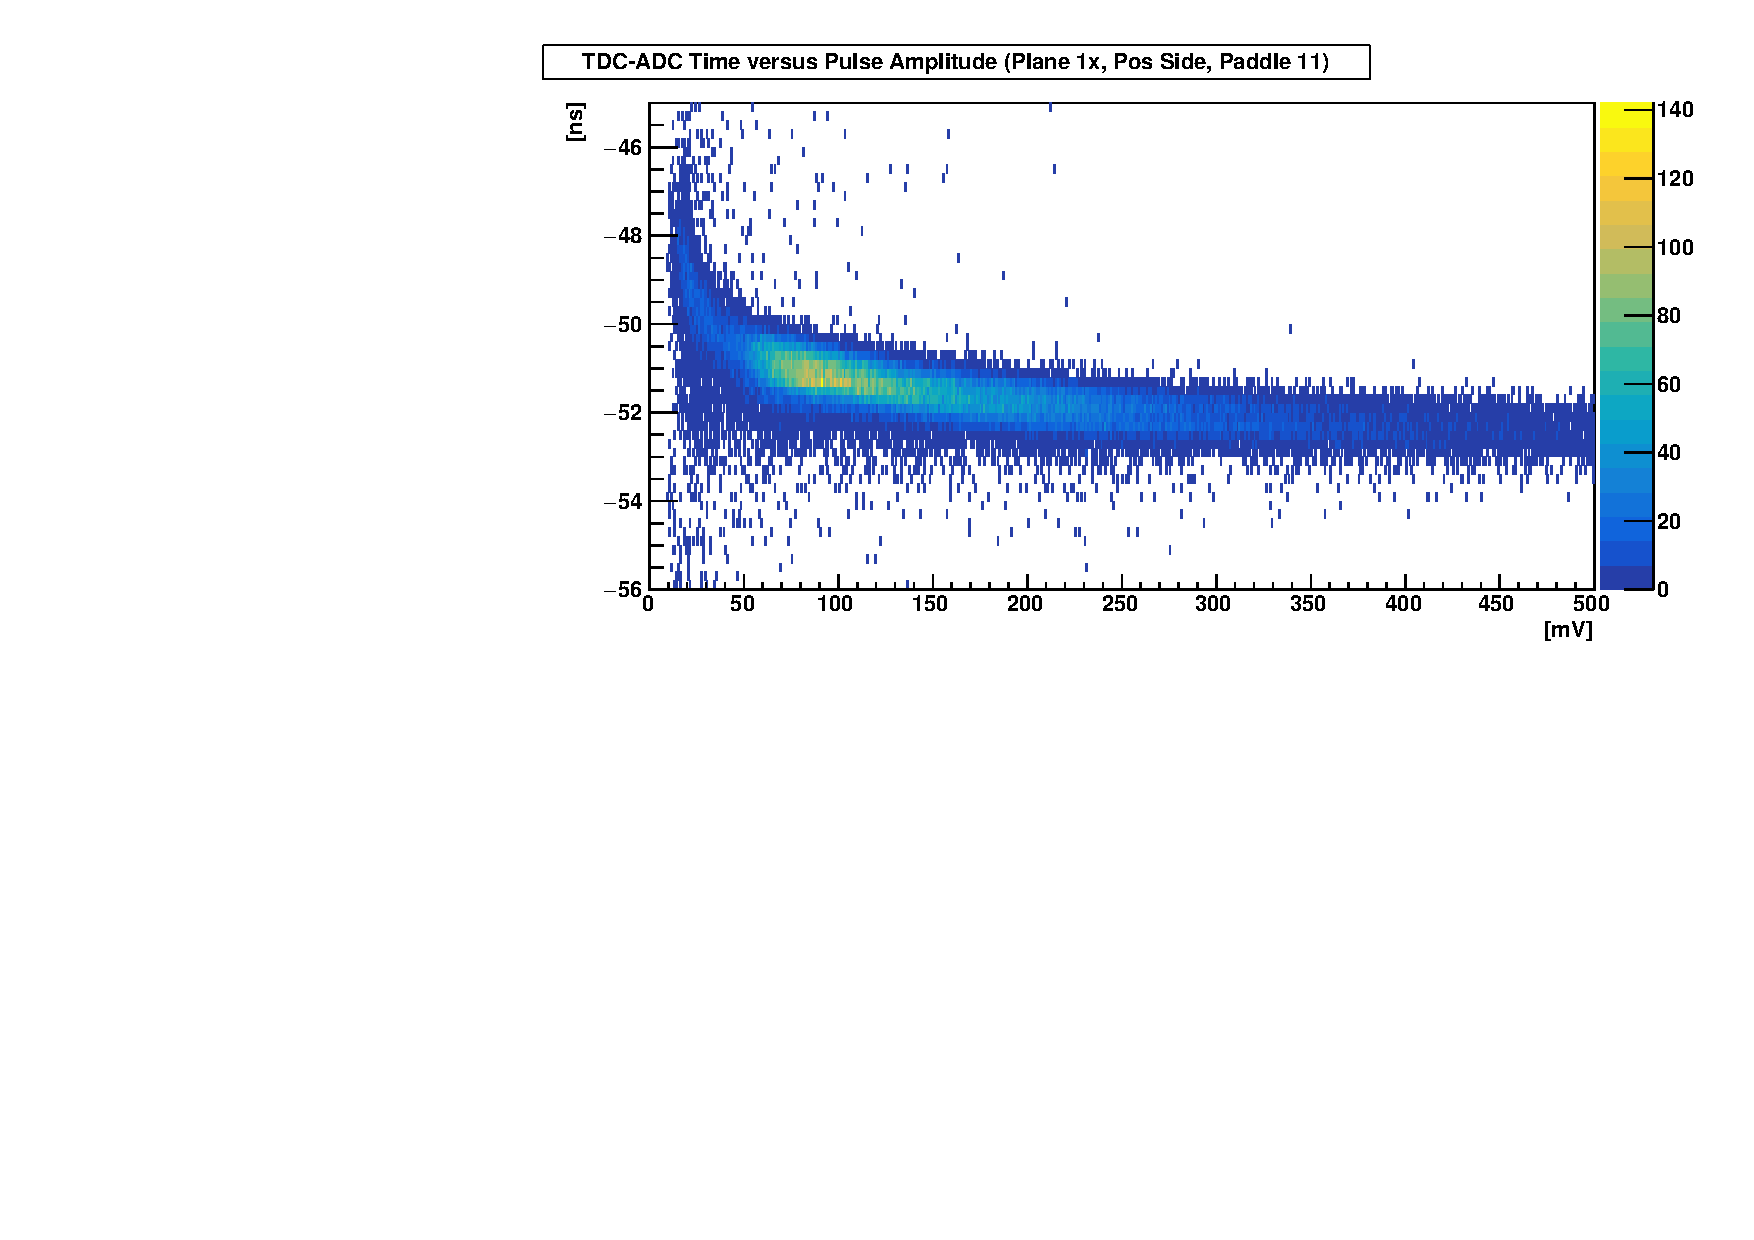
\includegraphics[width=1.0\textwidth]{chap4/plot_scripts/hodo_timewalk.pdf}
    \caption{
            A two dimensional histogram showing the difference between TDC
            and fADC pulse times as a function of fADC pulse amplitude.
            As shown in Fig~\ref{fig:pooser_timewalk}, smaller pulses cross a
            fixed threshold at a later time, leading to a delayed TDC time.
            }
    \label{fig:time_walk_histogram}
\end{figure}


    \item \textbf{Cable/light propagation time} $t_{cable}$, $t_{prop}$

Signals from the hodoscope travel through BNC cables from the detector hut
underground up to the electronics racks in the counting house above ground.
Differences in cable propagation time between the opposite ends of the paddles
need to be accounted for.
The timewalk-corrected TDC times for the $+$ and $-$ sides of a paddle are
the sum of the propagation time for the light through the paddle
and the propagation time through the cables,
$t^{\pm}=t^{\pm}_{prop}+t^{\pm}_{cable}$.
The difference between the $+$ and $-$ sides' times should be proportional to
the track's distance from the center of the paddle
% TODO: not actually $y$, but distance from center. clarify this.
(i.e. the $y$ coordinate for a horizontal paddle, $x$ for a vertical paddle).
If $v$ is the speed of light in the paddle, this difference is
$\Delta t = \frac{y}{v} + b$,
where $b$ is a parameter that captures the offset due to differences in cable
propagation time.
A linear fit of the time difference $\Delta t$ versus track distance from the
center of the paddle is used to extract the cable offset and light propagation
speed for each paddle.
The intercept $b$ is the cable propagation time correction $t_{cable}$
and the slope $1/v$ determines the light propagation time correction
$t^\pm_{prop}$.
For a horizontal paddle,
$t^\pm_{prop} = (\pm L_\pm \pm y_{hit})$
where $L_\pm$ is the $y$ coordinate of the ends of the paddle and
$y_{hit}$ is the $y$ coordinate of the particle's track projected to the
paddle's $z$ position.
The same formula holds for a vertical paddle, but using $L_\pm$ in the $x$
direction and $x_{hit}$ at the paddle's $z$ position.

    \item \textbf{Small perturbations} $t_{\lambda}$

This term corrects for small differences $\lambda$ in timing between planes.
Let $t_i$ be the time, corrected for timewalk and propagation time,
of a hit on a paddle in plane $i$,
and $D_{ij}$ be the distance between planes $i$ and $j$.
Then the difference between hits in these planes with small perturbations can
be expressed as
\begin{equation}
    (t_i+\lambda_i) - (t_j+\lambda_j) = \frac{D_{ij}}{v}
\end{equation}
or equivalently, defining a term $b_{ij}$,
\begin{equation}
    \lambda_i - \lambda_j = \frac{D_{ij}}{v} - (t_i - t_j) \equiv b_{ij}
\end{equation}

Generalizing this to all 6 combinations of differences between 4 planes, we can
set up a system of linear equations with coefficients $c_i,j=\pm1$ where $i$
represents one of the 6 plane combinations and $j$ is the ``absolute'' paddle
number.
Paddles are indexed with $j$ from 1 to the total number of paddles in the
4 planes.
In the HMS there are 52 total paddles, so the system of linear equations is

\begin{align}
    c_{1,1}\lambda_1 + c_{1,2}\lambda_2 + \cdots + c_{1,52}\lambda_52 &= b_{12} \\
    c_{2,1}\lambda_1 + c_{2,2}\lambda_2 + \cdots + c_{2,52}\lambda_52 &= b_{13} \\
    c_{3,1}\lambda_1 + c_{3,2}\lambda_2 + \cdots + c_{3,52}\lambda_52 &= b_{14} \\
    c_{4,1}\lambda_1 + c_{4,2}\lambda_2 + \cdots + c_{4,52}\lambda_52 &= b_{23} \\
    c_{5,1}\lambda_1 + c_{5,2}\lambda_2 + \cdots + c_{5,52}\lambda_52 &= b_{24} \\
    c_{6,1}\lambda_1 + c_{6,2}\lambda_2 + \cdots + c_{6,52}\lambda_52 &= b_{34} \\
\end{align}

or in matrix notation

\begin{gather}
    C\vec{\lambda}
    =
    \begin{bmatrix}
        c_{1,1} & c_{1,2} & \cdots & c_{1,52} \\
        c_{2,1} & c_{2,2} & \cdots & c_{2,52} \\
        c_{3,1} & c_{3,2} & \cdots & c_{3,52} \\
        c_{4,1} & c_{4,2} & \cdots & c_{4,52} \\
        c_{5,1} & c_{5,2} & \cdots & c_{5,52} \\
        c_{6,1} & c_{6,2} & \cdots & c_{6,52} \\
    \end{bmatrix}
    \left[ \begin{array}{c} \lambda_1 \\ \lambda_2 \\ \vdots \\ \lambda_{52} \end{array} \right]
    =
    \left[ \begin{array}{c} b_{12} \\ b_{13} \\ b_{14} \\ b_{23} \\ b_{24} \\ b_{34}  \end{array} \right]
\end{gather}

Solving this for all $\lambda$s requires accumulating statistics from a run with
many events $k$:
\begin{gather}
    C\vec{\lambda}
    =
    \begin{bmatrix}
        \sum_k c_{1,1} & \sum_k c_{1,2} & \cdots & \sum_k c_{1,52} \\
        \sum_k c_{2,1} & \sum_k c_{2,2} & \cdots & \sum_k c_{2,52} \\
        \sum_k c_{3,1} & \sum_k c_{3,2} & \cdots & \sum_k c_{3,52} \\
        \sum_k c_{4,1} & \sum_k c_{4,2} & \cdots & \sum_k c_{4,52} \\
        \sum_k c_{5,1} & \sum_k c_{5,2} & \cdots & \sum_k c_{5,52} \\
        \sum_k c_{6,1} & \sum_k c_{6,2} & \cdots & \sum_k c_{6,52} \\
    \end{bmatrix}
    \left[ \begin{array}{c} \lambda_1 \\ \lambda_2 \\ \vdots \\ \lambda_{52} \end{array} \right]
    =
    \left[ \begin{array}{c}  \sum_k b_{12} \\  \sum_k b_{13} \\  \sum_k b_{14} \\  \sum_k b_{23} \\  \sum_k b_{24} \\  \sum_k b_{34}  \end{array} \right]
\end{gather}

\textit{hcana} solves for $\vec{\lambda}$ using singular value
decomposition, yielding a set of corrections $t_\lambda = \lambda_i$ for every
paddle $i$.

% TODO: clarify that we only used timewalk corrections

\end{itemize}

\subsection{Drift Chambers} \label{sec:dc_calib}
When a charged particle passes through the drift chambers, it ionizes the gas
filling the chamber.
The electric field generated by the field wires causes the freed electrons to
drift toward sense wires over a ``drift time'' $t_D$.
The sense wires are read out by discriminators fed into TDC channels.
Knowledge of which wires in each plane have been fired permits coarse track
reconstruction.
Finer resolution can be achieved by using the drift time to estimate a drift
distance $d_D$, the distance from the wire at which the ionization occurred.


Assuming the events used for calibration illuminate the detector uniformly
and that the drift velocity is uniform across the detector, the relationship
between drift distance and drift time $t_D$ is
\begin{equation}
    d_D (\tau=t_D) = \frac{\Delta}{2}
                     \frac{\int_{t_0}^{t_D<t_{max}} F(\tau) d\tau}
                          {\int_{t_0}^{t_{max}} F(\tau) d\tau}
\end{equation}

where $F(\tau)$ is the distribution of drift times.
The times $t_0$ and $t_{max}$ are the minimum and maximum drift times,
determined by the cell spacing and drift velocity.
They are extracted from the distribution $F(\tau)$.
The constant $\Delta/2$ ensures this expression respects the limiting cases of
particles passing immediately adjacent to a sense wire or exactly between
two sense wires.


The TDCs have a finite resolution, so these integrals are in reality actually
sums over bins $F_i$ with widths $\Delta\tau$,
\begin{align} \label{eqn:drift_distance}
    d_D (\tau=t_D) &= \frac{\Delta}{2}
                      \frac{\sum_{i=0}^{n_{max}<N} F_i \Delta\tau}
                           {\sum_{i=0}^{N} F_i \Delta\tau} \\
                 &= \frac{\Delta}{2}
                    \frac{1}{N}\sum_{i=0}^{n_{max}} F_i
\end{align}
where $i$ is the bin index,
$n$ is the index of the bin in which drift time $t_D$ lies,
and $N$ is the index of the maximum drift time.


The first step in calibrating the drift chambers is determining a $t_0$ for
every wire.
This is done by finding the point at which a linear fit of the lower range of
the drift time spectrum to cross the x axis, as shown in
Fig~\ref{fig:drift_time_fit}.
If there are insufficient per-wire statistics to obtain a good fit,
the distribution for all 16 wires connected to a card may be used instead to
obtain a per-card $t_0$.

\begin{figure}[!h]
    \centering
    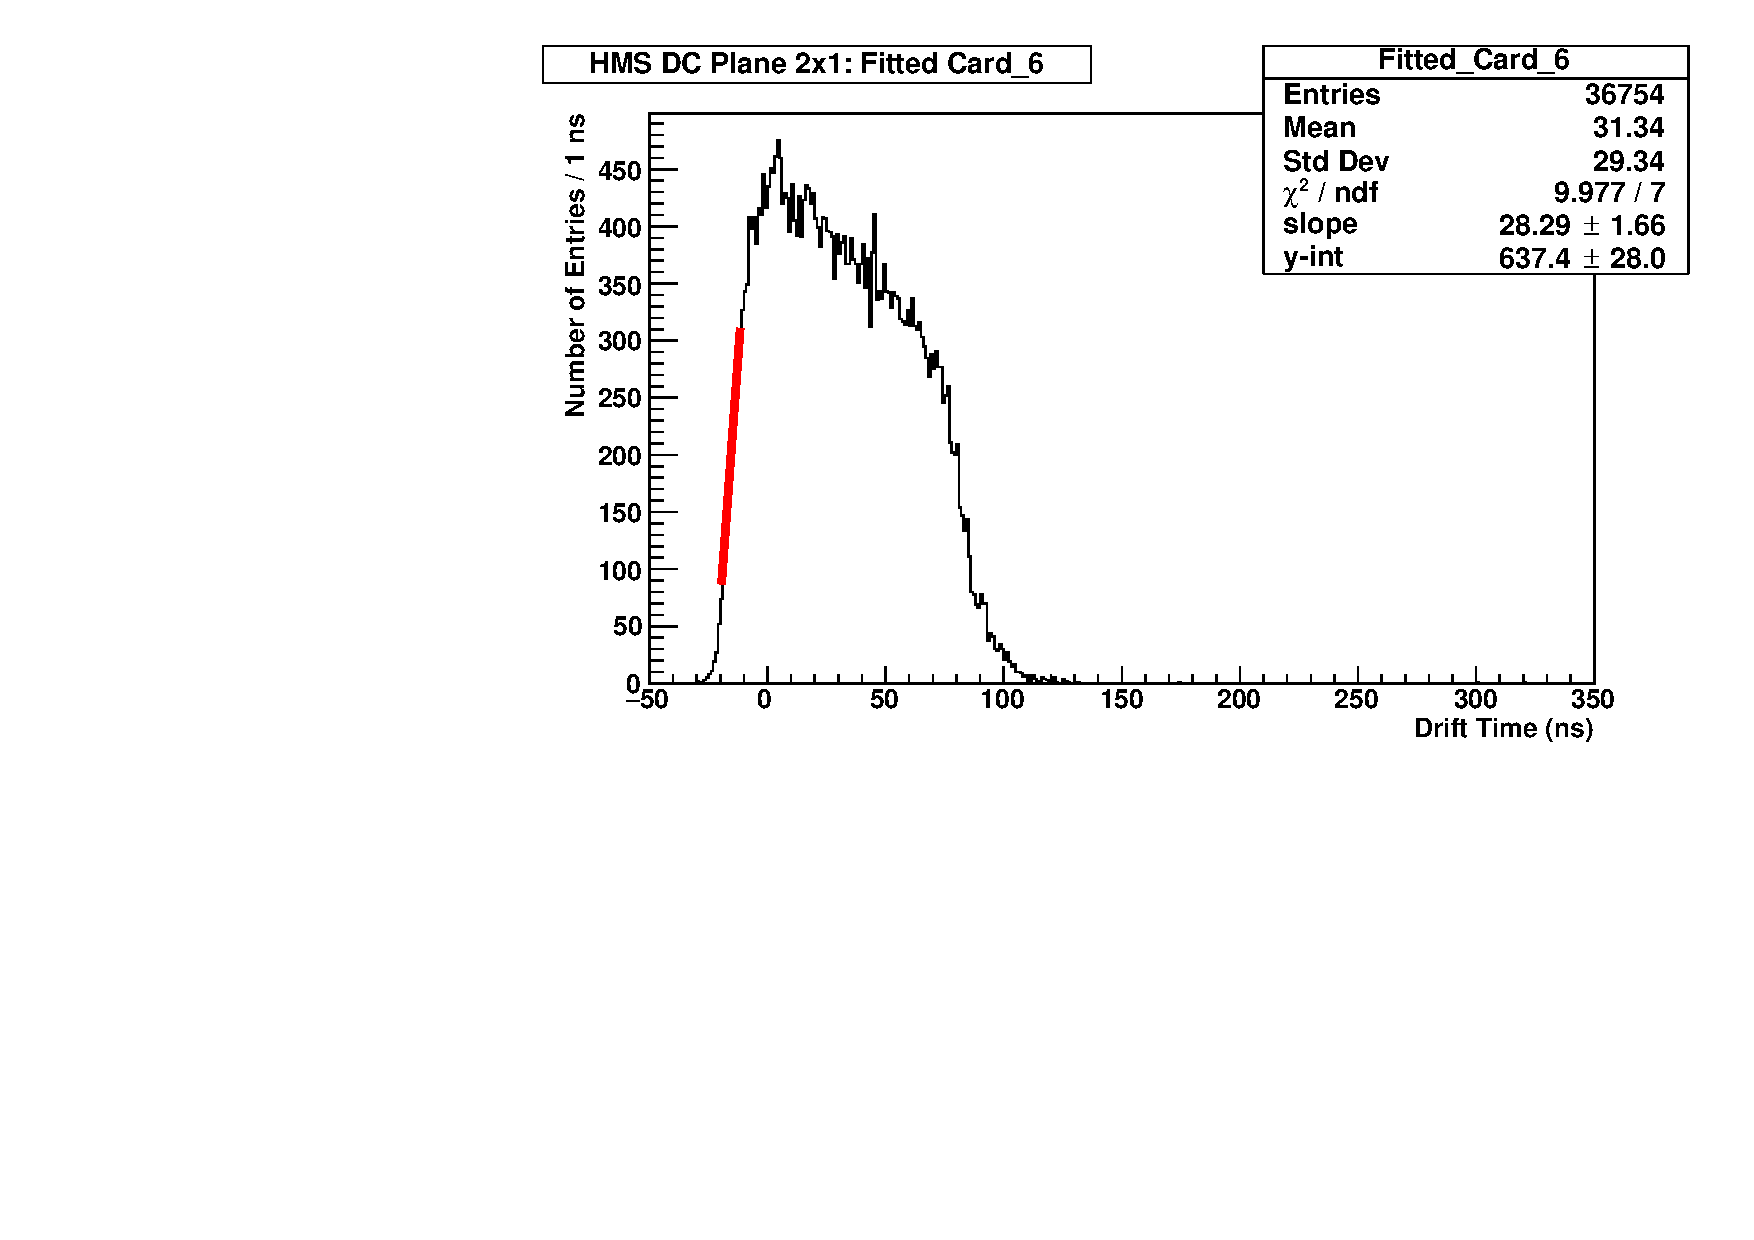
\includegraphics[width=0.8\textwidth]{chap4/drift_time_fit.pdf}
    \caption{
            The distribution of drift times for one card in the HMS 2x1 plane.
            The red line is a linear fit to the range corresponding to 20--60\%
            of the maximum bin content.
            The x-intercept of the fit is used as the offset $t_0$ for all
            wires in the card.
            }
    \label{fig:drift_time_fit}
\end{figure}

The calibration script first generates a histogram of drift times with bins of
width \SI{1}{\nano\second}
and finds the bin in the histogram containing the maximum number of entries.
A linear fit is then performed over the bins corresponding to 20--60\% of the
maximum bin content.
The x-intercept of this fit yields $t_0$, which can then be used to create a
lookup table using equation~\ref{eqn:drift_distance}.
An example of the distribution of uncorrected and corrected drift times is
shown in Fig~\ref{fig:drift_th2s}.

\begin{figure}[ht]
    \centering
    \begin{subfigure}[b]{0.8\textwidth}
        \centering
        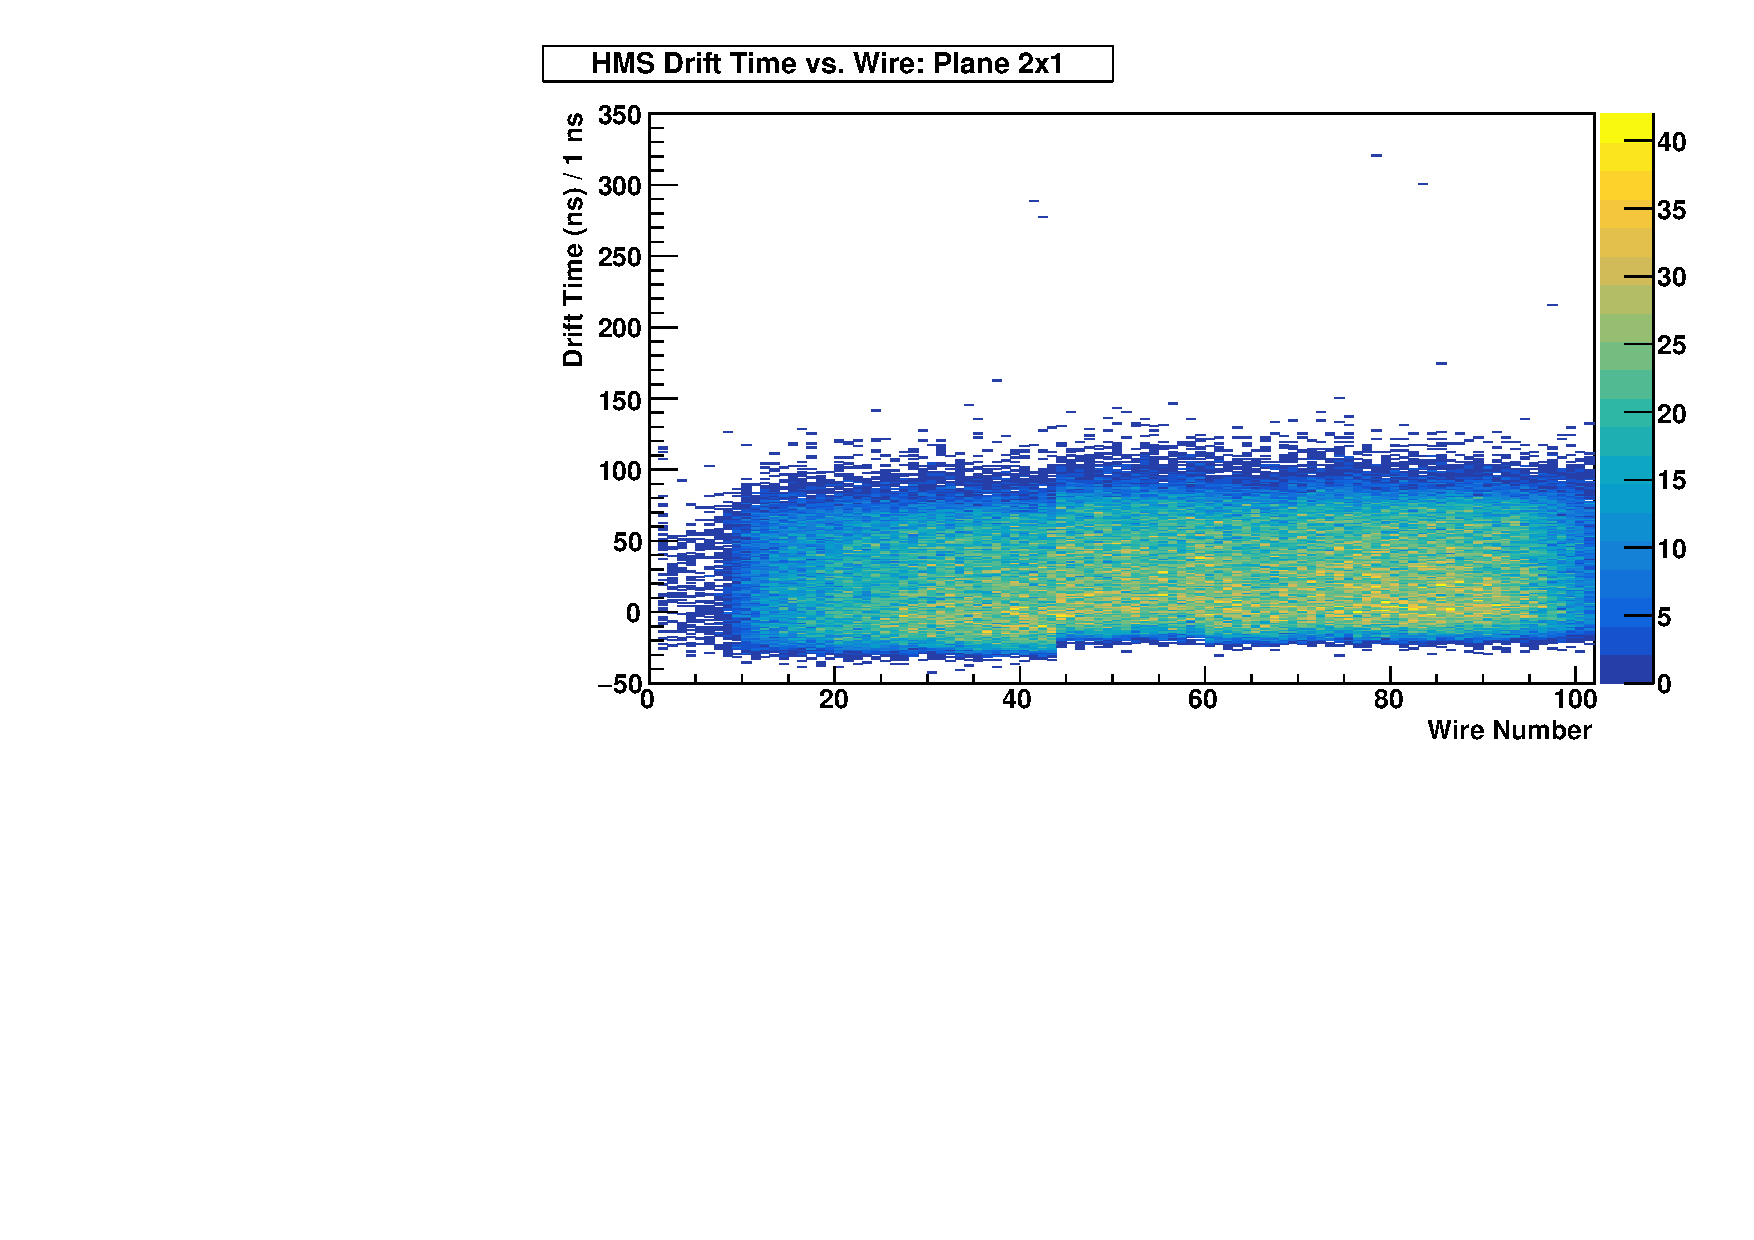
\includegraphics[width=\textwidth]{chap4/uncorrected_drift_times_2x1_TH2.pdf}
        \caption{Uncorrected drift times.}
        \label{fig:uncorrected_drift_th2}
    \end{subfigure}
    \vspace{0.1cm}
    \\
    \begin{subfigure}[b]{0.8\textwidth}
        \centering
        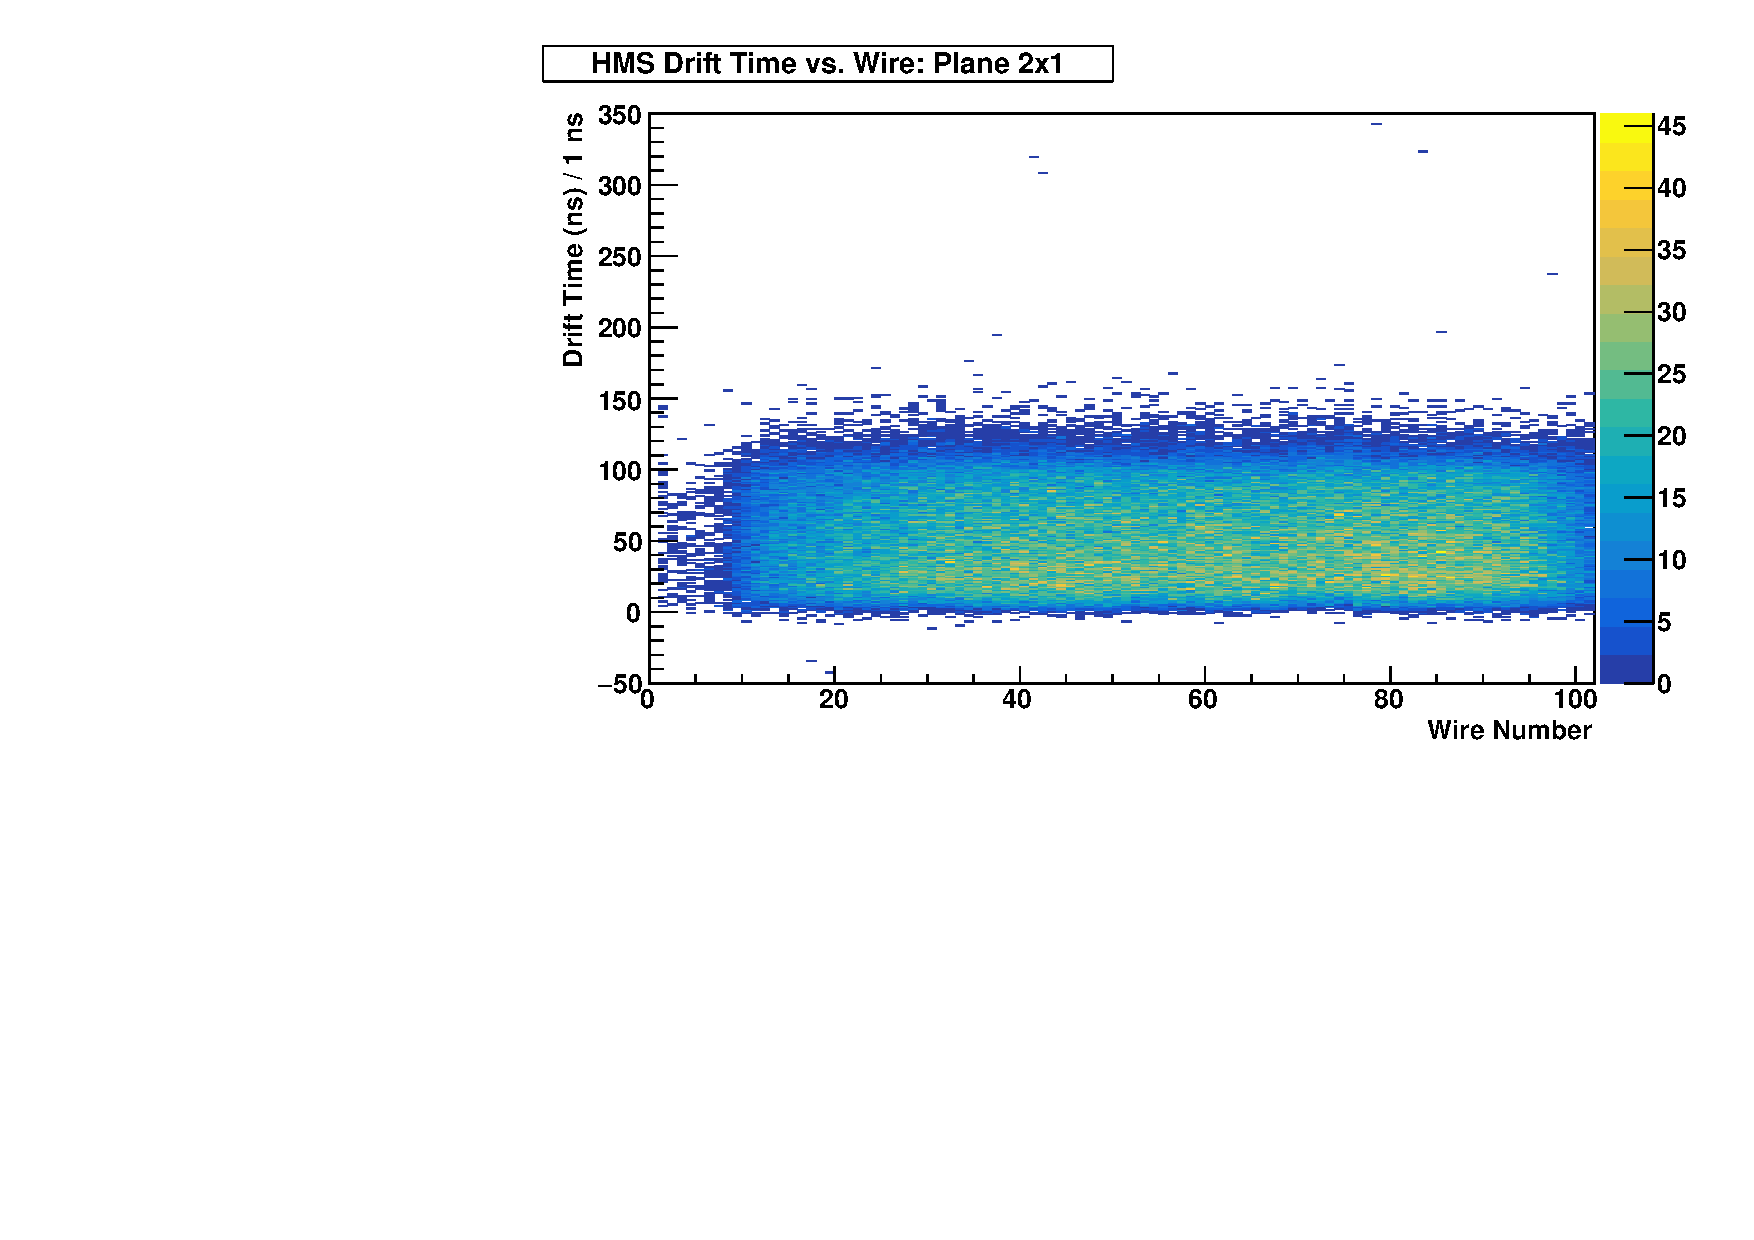
\includegraphics[width=\textwidth]{chap4/corrected_drift_times_2x1_TH2.pdf}
        \caption{Corrected drift times.}
        \label{fig:corrected_drift_th2}
    \end{subfigure}
    \caption{Two dimensional histograms of wire drift times for the HMS 2x1 plane,
             before (a) and after (b) $t_0$ correction.}
    \label{fig:drift_th2s}
\end{figure}

% TODO residuals

\subsection{Cherenkovs}

The calibration procedure for all threshold Cherenkov counters in both
spectrometers involves extracting per-PMT conversion factors $\alpha_i$ to
convert ADC pulse integrals to a number of photoelectrons.
The number of photoelectrons collected by PMT $i$ is $n_i=\alpha_iq_i$ where
$q_i$ is the pulse integral recorded for PMT $i$'s channel in the DAQ.


For the HMS Cherenkov, it is relatively straightforward to identify the single
photoelectron peak in histograms of each PMT's pedestal-subtracted pulse
integrals.
This peak can be fit to a Gaussian with mean $\mu$ and standard deviation
$\sigma$.
The mean $\mu$ is the number of \si{\pico\coulomb} generated by one
photoelectron.
The conversion factor is then $\alpha_i=1/\mu$.

\begin{figure}[!h]
    \centering
    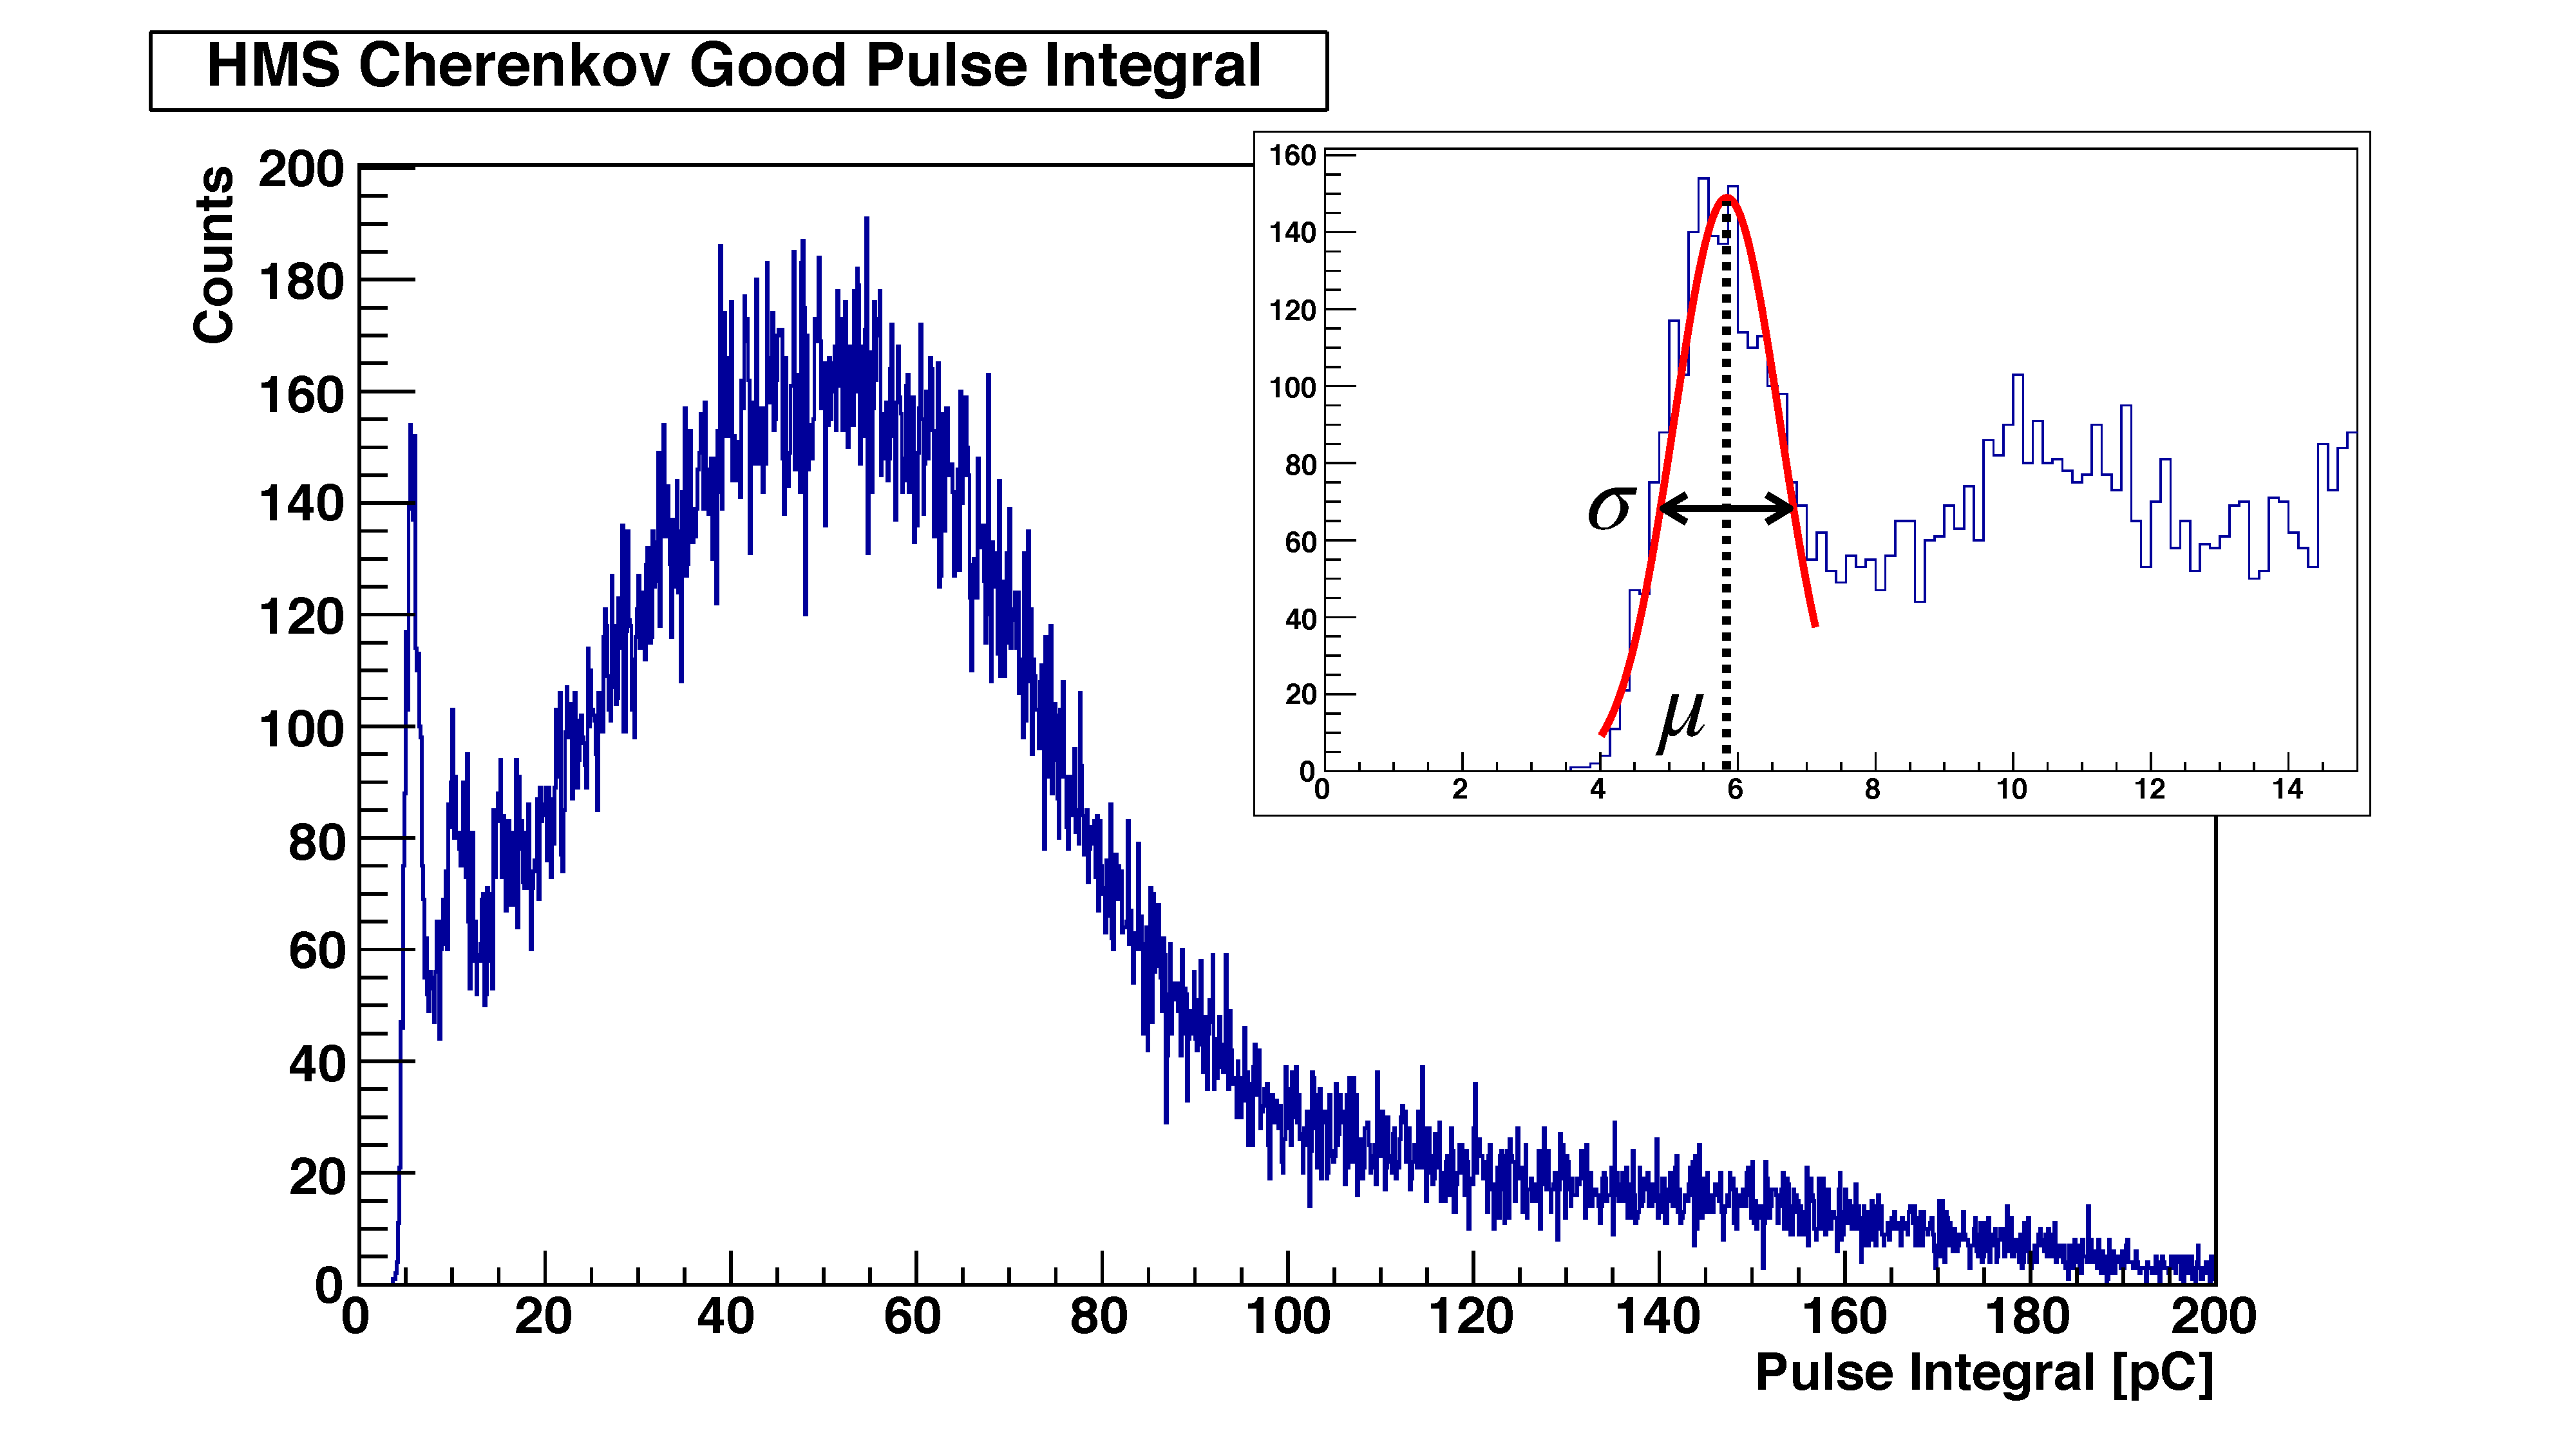
\includegraphics[width=0.8\textwidth]{chap4/plot_scripts/hcer_pulseint_composite.pdf}
    \caption{
            The distribution of pulse integrals in one PMT of the HMS
            Cherenkov.
            The single-photoelectron peak can be seen around
            \SI{6}{\pico\coulomb}, the two-photoelectron peak can be faintly
            seen around \SI{12}{\pico\coulomb}.
            The inset plot shows a Gaussian fit to the the single-photoelectron
            peak.
            }
    \label{fig:normalized_edep}
\end{figure}

Finding this peak for the SHMS Noble Gas Cherenkov has proved difficult, so a
second method was developed.
Events where an electron's Cherenkov radiation is focused on a single PMT are
selected by cutting on
calorimeter track-normalized energy approximately equal to 1,
track position in the PMT's quadrant at the mirror plane,
and low pulse integral in the other PMTs.
The histograms of pulse integrals for these events are again fit with a
Gaussian, from which the number of photoelectrons can be estimated to be
$N_{PE}=(\mu/\sigma)^2$.
The location of the single photoelectron peak in this histogram should then
be $\mu/N_{PE}=\mu/(\mu/\sigma)^2=\sigma^2/\mu$.
The conversion factor is $\alpha_i=\mu/\sigma^2$.


\subsection{Calorimeters}
% Plots to make for a run with good statistics
% etottracknorm
% T->Draw("H.cal.etottracknorm>>h(300,0,1.5)","H.cal.etottracknorm>0")
% shower vs preshower
% T->Draw("H.cal.etottracknorm-H.cal.eprtracknorm:H.cal.eprtracknorm>>h(100,0,1.0,120,0,1.2)","","colz")
% delta vs etottracknorm; should be vertical at 1
% T->Draw("H.gtr.dp:H.cal.etottracknorm>>h(300,0,1.5,90,-15,15)","","colz")

% Optimzation problem for calibration summarized in these slides,
% but it seems like the attenuation correction for the track y position
% is not described here.
% https://hallaweb.jlab.org/data_reduc/AnaWork2015/HMS_Calorimeter_in_HCANA.pdf

% Looking at hcana source:
% COARSE PROCESS:
%  The conversion factor is a "gain" which is the product:
%  gain = cal_{something}_cal_const[n] * cal_{something}_gain_cor[n]
%  The cal_consts are currently all 0.001. Seems silly but ok.
%
% FINE PROCESS:
%  There's a few Ycor functions in THcShower.h
%   They use parameters like cal_a_cor and a function like TMath::Exp(y/fAcor)/(1. + y*y/fBcor)
%   The parameters are in p(h)cal_geom.param.
%   Probably measured by someone like Vardan
% For reference:
% hcal_a_cor = 200.
% hcal_b_cor = 8000.
% hcal_c_cor = 64.36, 64.36
% hcal_d_cor = 1.66,  1.66
% pcal_a_cor = 106.73
% pcal_b_cor = 2.329
% pcal_c_cor = 0 0
% pcal_d_cor = 0 0

Energy deposited by particles in the calorimeters is reconstructed by
converting ADC pulse integrals recorded for each PMT to
the equivalent amount of energy converted into light collected by the PMTs.
Accurate reconstruction requires accounting for both
variations in PMT gain
and
attenuation as light propagates through the blocks.
The PMTs were matched at the hardware level to have equal output amplitudes, so
as to make the calorimeter pretrigger efficiencies as uniform as possible over
the spectrometers' acceptances.
The energy $e_i$ deposited in channel $i$ is estimated by
$e_i = \alpha_i q_i f(y)$
where
$\alpha_i$ is the channel's calibration constant,
$q_i$ is the pulse integral recorded by the DAQ,
and $f(y)$ is an attenuation correction.

\textit{hcana} first converts pulse integrals to equivalent energy with a
per-PMT conversion factor in the \texttt{CoarseProcess()} loop, and then
in the \texttt{FineProcess()} loop applies an attenuation correction
to each layer's reconstructed energy.
This correction is a function of the track's horizontal $y$ coordinate, so the
blocks in the SHMS shower array, which run roughly parallel to the $z$
coordinate, receive no attenuation correction.

The correction for blocks in HMS layers A and B, which have PMTs on both sides is:
\begin{equation}
    f_{\pm}(y) = \frac{C \pm y}{C \pm \frac{y}{D}}
\end{equation}

The correction for blocks in HMS layers C and D, which have PMTs on only one side, is:
\begin{equation}
    f(y) = \frac{e^{\frac{y}{A}}}{1 + \frac{y^2}{B}}
\end{equation}

The correction for blocks in the SHMS preshower layer is:
\begin{equation}
    f(y) = \frac{1}{1 + \left(\frac{\abs{y}}{A}\right)^B}
\end{equation}

The parameters $A$, $B$, $C$, and $D$ in the above expressions were determined
based on measurements of light transmittance made with a
spectrophotometer~\cite{Mkrtchyan_2012}.


Determining the calibration coefficients is a constrained optimization
problem~\cite{Amatuni, Vardan_cal_slides}.
Let $N$ be the number of PMTs in the calorimeter,
$q = (q_1, \cdots, q_N)^T$ their ADC pulse integrals,
$\alpha = (\alpha_1, \cdots, \alpha_N)^T$ their calibration constants,
$e_0 = E(e)$ the mean of particle energies $e$ obtained from the track reconstruction,
and $q_0 = E(q)$ the mean ADC pulse integral.
Then $e_R = \alpha^T q$ is the reconstructed particle energy.
To determine $\alpha$, the variance of the reconstructed energies with respect
to the track energies should be minimized.
That is, $E(e_R-e)^2$ should be minimized subject to the constraint
$\alpha^T q_0=e_0$.

The optimized calibration constants are
\begin{equation}
    \alpha_C = \frac{e_0 - \alpha_U^T q_0}{q_0^T Q^{-1} q_0} Q^{-1} q_0 + \alpha_U
\end{equation}
where $\alpha_U = Q^{-1}q_e$ are unconstrained calibration constants obtained
from the correlation matrix $Q=E(qq^T)$ and $q_e=E(eq)$.

The distribution of track-normalized energy deposition for this experiment's
data taken at $Q^2=\SI{8.0}{\giga\electronvolt}$ with the liquid hydrogen
target is shown in Fig~\ref{fig:normalized_edep}.
The red histogram represents events that did not fire the HMS Cherenkov.
Pions should not fire the Cherenkov and should deposit very little of their
energy in the calorimeter as a fraction of their momentum, which leads to the
red distribution being skewed to the left in this figure.
The blue histogram represents events that fired the HMS Cherenkov.
Electrons should fire the Cherenkov and deposit all of their energy in the
calorimeter, which leads to the peak around $E_{dep}/p=1$.
The blue events at low $E_{dep}/p$ may be pions that ``accidentally'' fired the
Cherenkov via knock-on electrons.

\begin{figure}[!h]
    \centering
    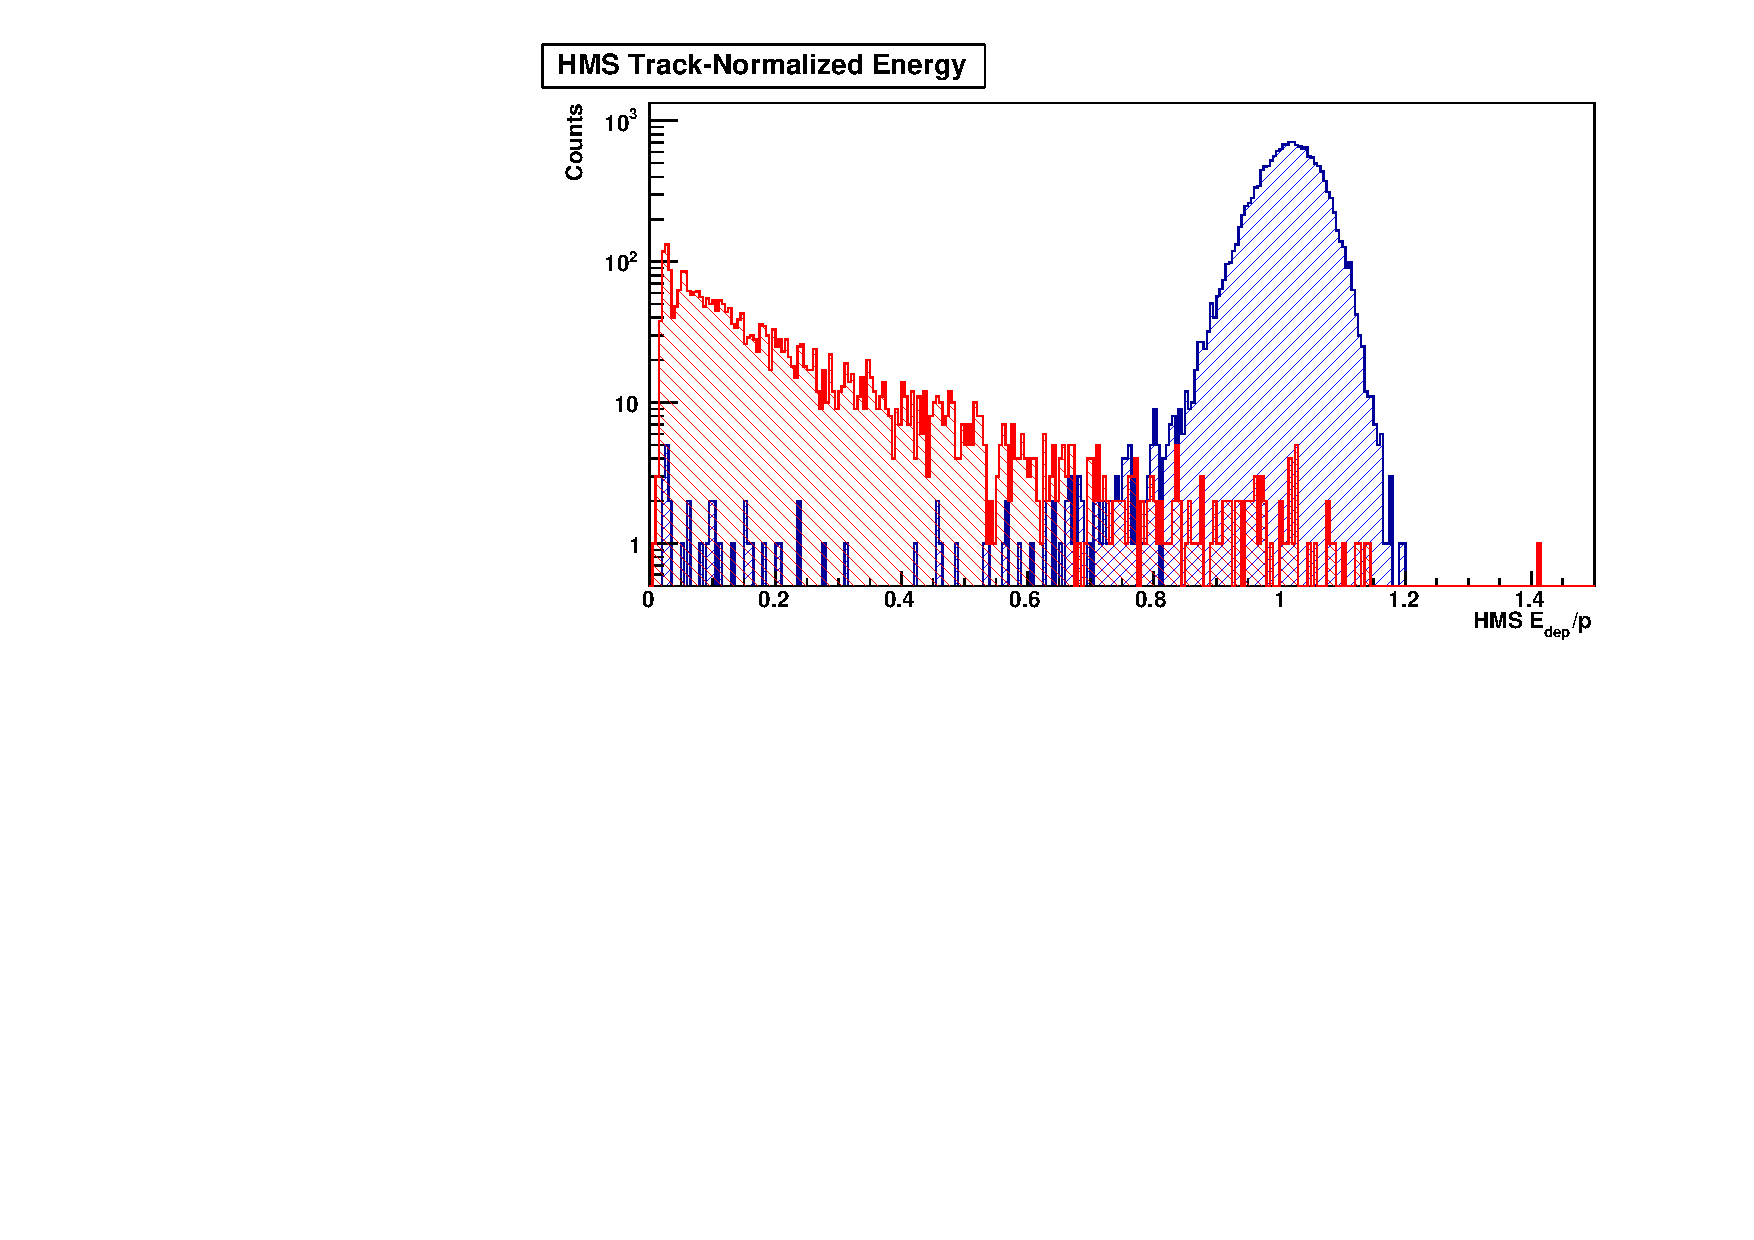
\includegraphics[width=0.8\textwidth]{chap4/plot_scripts/normalized_edep_lh2_q2_8.pdf}
    \caption{
            Track-normalized energy deposition for this experiment's
            $Q^2=\SI{8.0}{\giga\electronvolt}$ hydrogen data.
            The blue (red) histogram represents events that did (did not) fire the HMS Cherenkov.
            }
    \label{fig:normalized_edep}
\end{figure}

A two-dimensional histogram of HMS delta and track-normalized energy deposition
is shown in Fig~\ref{fig:delta_vs_edep}, illustrating the quality of the
calibration.
The blob around $E_{dep}/p=1$ primarily contains electrons, and the blob at
left contains pions.

\begin{figure}[!h]
    \centering
    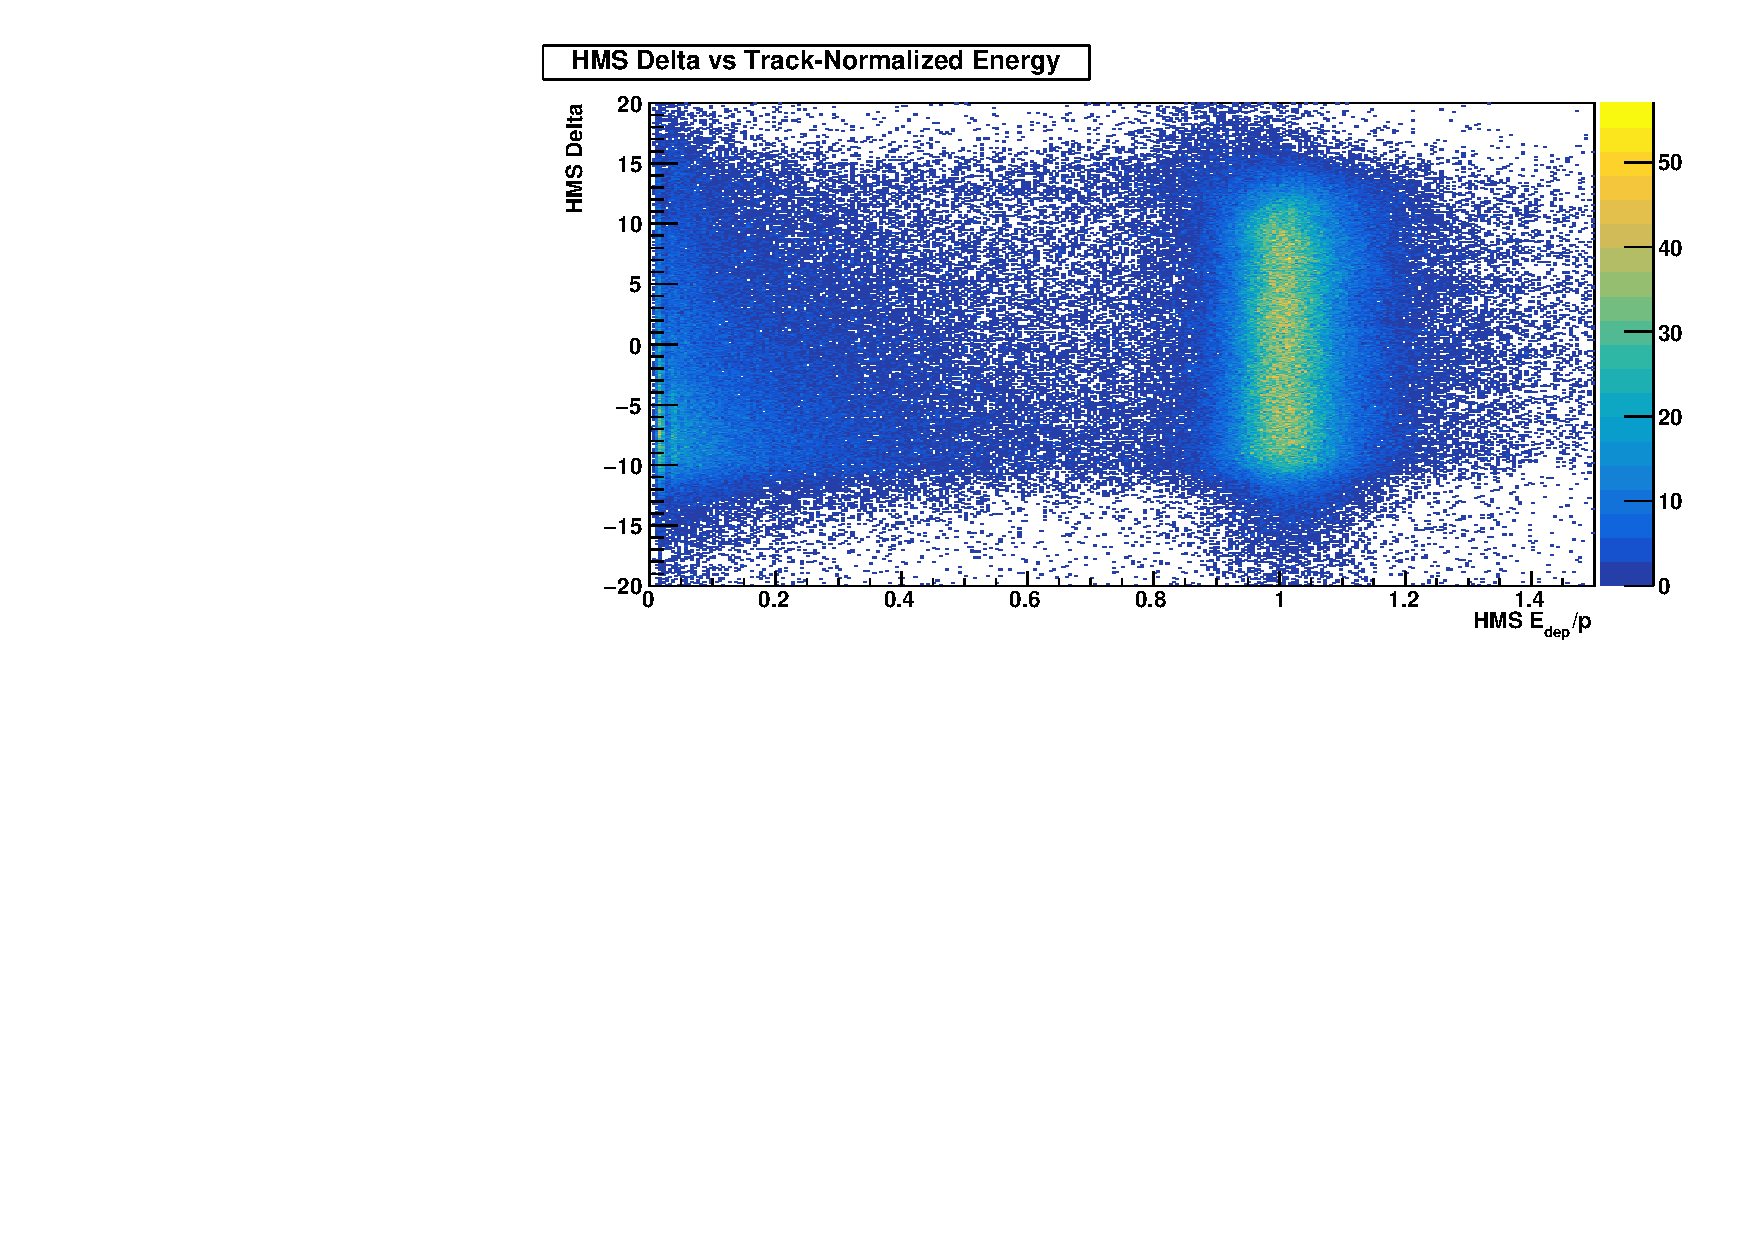
\includegraphics[width=0.8\textwidth]{chap4/plot_scripts/delta_vs_normalized_edep.pdf}
    \caption{
            A two-dimensional histogram of HMS delta versus track-normalized
            energy deposition in the HMS calorimeter.
            }
    \label{fig:delta_vs_edep}
\end{figure}

